\documentclass[twoside]{book}

% Packages required by doxygen
\usepackage{fixltx2e}
\usepackage{calc}
\usepackage{doxygen}
\usepackage[export]{adjustbox} % also loads graphicx
\usepackage{graphicx}
\usepackage[utf8]{inputenc}
\usepackage{makeidx}
\usepackage{multicol}
\usepackage{multirow}
\PassOptionsToPackage{warn}{textcomp}
\usepackage{textcomp}
\usepackage[nointegrals]{wasysym}
\usepackage[table]{xcolor}

% Font selection
\usepackage[T1]{fontenc}
\usepackage[scaled=.90]{helvet}
\usepackage{courier}
\usepackage{amssymb}
\usepackage{sectsty}
\renewcommand{\familydefault}{\sfdefault}
\allsectionsfont{%
  \fontseries{bc}\selectfont%
  \color{darkgray}%
}
\renewcommand{\DoxyLabelFont}{%
  \fontseries{bc}\selectfont%
  \color{darkgray}%
}
\newcommand{\+}{\discretionary{\mbox{\scriptsize$\hookleftarrow$}}{}{}}

% Page & text layout
\usepackage{geometry}
\geometry{%
  a4paper,%
  top=2.5cm,%
  bottom=2.5cm,%
  left=2.5cm,%
  right=2.5cm%
}
\tolerance=750
\hfuzz=15pt
\hbadness=750
\setlength{\emergencystretch}{15pt}
\setlength{\parindent}{0cm}
\setlength{\parskip}{3ex plus 2ex minus 2ex}
\makeatletter
\renewcommand{\paragraph}{%
  \@startsection{paragraph}{4}{0ex}{-1.0ex}{1.0ex}{%
    \normalfont\normalsize\bfseries\SS@parafont%
  }%
}
\renewcommand{\subparagraph}{%
  \@startsection{subparagraph}{5}{0ex}{-1.0ex}{1.0ex}{%
    \normalfont\normalsize\bfseries\SS@subparafont%
  }%
}
\makeatother

% Headers & footers
\usepackage{fancyhdr}
\pagestyle{fancyplain}
\fancyhead[LE]{\fancyplain{}{\bfseries\thepage}}
\fancyhead[CE]{\fancyplain{}{}}
\fancyhead[RE]{\fancyplain{}{\bfseries\leftmark}}
\fancyhead[LO]{\fancyplain{}{\bfseries\rightmark}}
\fancyhead[CO]{\fancyplain{}{}}
\fancyhead[RO]{\fancyplain{}{\bfseries\thepage}}
\fancyfoot[LE]{\fancyplain{}{}}
\fancyfoot[CE]{\fancyplain{}{}}
\fancyfoot[RE]{\fancyplain{}{\bfseries\scriptsize Generated by Doxygen }}
\fancyfoot[LO]{\fancyplain{}{\bfseries\scriptsize Generated by Doxygen }}
\fancyfoot[CO]{\fancyplain{}{}}
\fancyfoot[RO]{\fancyplain{}{}}
\renewcommand{\footrulewidth}{0.4pt}
\renewcommand{\chaptermark}[1]{%
  \markboth{#1}{}%
}
\renewcommand{\sectionmark}[1]{%
  \markright{\thesection\ #1}%
}

% Indices & bibliography
\usepackage{natbib}
\usepackage[titles]{tocloft}
\setcounter{tocdepth}{3}
\setcounter{secnumdepth}{5}
\makeindex

% Hyperlinks (required, but should be loaded last)
\usepackage{ifpdf}
\ifpdf
  \usepackage[pdftex,pagebackref=true]{hyperref}
\else
  \usepackage[ps2pdf,pagebackref=true]{hyperref}
\fi
\hypersetup{%
  colorlinks=true,%
  linkcolor=blue,%
  citecolor=blue,%
  unicode%
}

% Custom commands
\newcommand{\clearemptydoublepage}{%
  \newpage{\pagestyle{empty}\cleardoublepage}%
}

\usepackage{caption}
\captionsetup{labelsep=space,justification=centering,font={bf},singlelinecheck=off,skip=4pt,position=top}

%===== C O N T E N T S =====

\begin{document}

% Titlepage & ToC
\hypersetup{pageanchor=false,
             bookmarksnumbered=true,
             pdfencoding=unicode
            }
\pagenumbering{alph}
\begin{titlepage}
\vspace*{7cm}
\begin{center}%
{\Large System Programming }\\
\vspace*{1cm}
{\large Generated by Doxygen 1.8.13}\\
\end{center}
\end{titlepage}
\clearemptydoublepage
\pagenumbering{roman}
\tableofcontents
\clearemptydoublepage
\pagenumbering{arabic}
\hypersetup{pageanchor=true}

%--- Begin generated contents ---
\chapter{Class Index}
\section{Class List}
Here are the classes, structs, unions and interfaces with brief descriptions\+:\begin{DoxyCompactList}
\item\contentsline{section}{\hyperlink{structTie}{Tie$<$ T, N, M $>$} }{\pageref{structTie}}{}
\end{DoxyCompactList}

\chapter{File Index}
\section{File List}
Here is a list of all files with brief descriptions\+:\begin{DoxyCompactList}
\item\contentsline{section}{src/source/3/\hyperlink{c__m__t_8h}{c\+\_\+m\+\_\+t.\+h} }{\pageref{c__m__t_8h}}{}
\item\contentsline{section}{src/source/3/\hyperlink{main_8cpp}{main.\+cpp} }{\pageref{main_8cpp}}{}
\end{DoxyCompactList}

\chapter{Class Documentation}
\hypertarget{structTie}{}\section{Tie$<$ T, N, M $>$ Struct Template Reference}
\label{structTie}\index{Tie$<$ T, N, M $>$@{Tie$<$ T, N, M $>$}}


{\ttfamily \#include $<$c\+\_\+m\+\_\+t.\+h$>$}

\subsection*{Public Member Functions}
\begin{DoxyCompactItemize}
\item 
\hyperlink{structTie_a58df4b2dbd5e7e5be53529d0daa89ca1}{Tie} (std\+::array$<$ T $\ast$, M $>$ arr)
\item 
void \hyperlink{structTie_af835eefa6c2e6208589721587d8f743d}{operator=} (const std\+::array$<$ T, N $\ast$M $>$ \&rhs)
\end{DoxyCompactItemize}
\subsection*{Public Attributes}
\begin{DoxyCompactItemize}
\item 
std\+::array$<$ T $\ast$, M $>$ \hyperlink{structTie_a787e11998c210d1f1019ad3aee9adf82}{tuple}
\end{DoxyCompactItemize}


\subsection{Constructor \& Destructor Documentation}
\mbox{\Hypertarget{structTie_a58df4b2dbd5e7e5be53529d0daa89ca1}\label{structTie_a58df4b2dbd5e7e5be53529d0daa89ca1}} 
\index{Tie@{Tie}!Tie@{Tie}}
\index{Tie@{Tie}!Tie@{Tie}}
\subsubsection{\texorpdfstring{Tie()}{Tie()}}
{\footnotesize\ttfamily template$<$class T , int N, int M$>$ \\
\hyperlink{structTie}{Tie}$<$ T, N, M $>$\+::\hyperlink{structTie}{Tie} (\begin{DoxyParamCaption}\item[{std\+::array$<$ T $\ast$, M $>$}]{arr }\end{DoxyParamCaption})\hspace{0.3cm}{\ttfamily [inline]}}



\subsection{Member Function Documentation}
\mbox{\Hypertarget{structTie_af835eefa6c2e6208589721587d8f743d}\label{structTie_af835eefa6c2e6208589721587d8f743d}} 
\index{Tie@{Tie}!operator=@{operator=}}
\index{operator=@{operator=}!Tie@{Tie}}
\subsubsection{\texorpdfstring{operator=()}{operator=()}}
{\footnotesize\ttfamily template$<$class T , int N, int M$>$ \\
void \hyperlink{structTie}{Tie}$<$ T, N, M $>$\+::operator= (\begin{DoxyParamCaption}\item[{const std\+::array$<$ T, N $\ast$M $>$ \&}]{rhs }\end{DoxyParamCaption})\hspace{0.3cm}{\ttfamily [inline]}}



\subsection{Member Data Documentation}
\mbox{\Hypertarget{structTie_a787e11998c210d1f1019ad3aee9adf82}\label{structTie_a787e11998c210d1f1019ad3aee9adf82}} 
\index{Tie@{Tie}!tuple@{tuple}}
\index{tuple@{tuple}!Tie@{Tie}}
\subsubsection{\texorpdfstring{tuple}{tuple}}
{\footnotesize\ttfamily template$<$class T , int N, int M$>$ \\
std\+::array$<$T$\ast$, M$>$ \hyperlink{structTie}{Tie}$<$ T, N, M $>$\+::tuple}



The documentation for this struct was generated from the following file\+:\begin{DoxyCompactItemize}
\item 
src/source/3/\hyperlink{c__m__t_8h}{c\+\_\+m\+\_\+t.\+h}\end{DoxyCompactItemize}

\chapter{File Documentation}
\hypertarget{c__m__t_8h}{}\section{src/source/3/c\+\_\+m\+\_\+t.h File Reference}
\label{c__m__t_8h}\index{src/source/3/c\+\_\+m\+\_\+t.\+h@{src/source/3/c\+\_\+m\+\_\+t.\+h}}
{\ttfamily \#include $<$iostream$>$}\newline
{\ttfamily \#include $<$cstdarg$>$}\newline
{\ttfamily \#include $<$array$>$}\newline
{\ttfamily \#include $<$gtest/gtest.\+h$>$}\newline
Include dependency graph for c\+\_\+m\+\_\+t.\+h\+:
\nopagebreak
\begin{figure}[H]
\begin{center}
\leavevmode
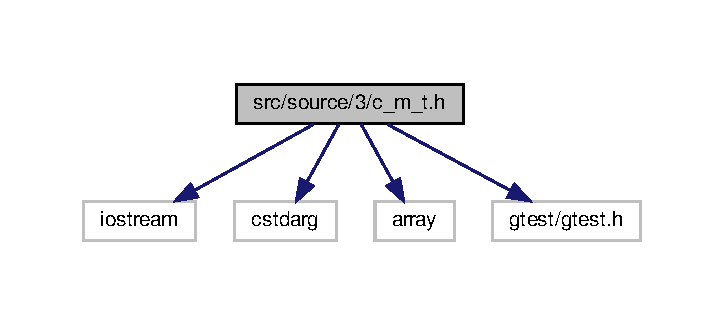
\includegraphics[width=348pt]{c__m__t_8h__incl}
\end{center}
\end{figure}
This graph shows which files directly or indirectly include this file\+:
\nopagebreak
\begin{figure}[H]
\begin{center}
\leavevmode
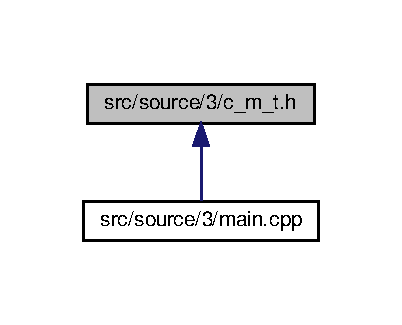
\includegraphics[width=193pt]{c__m__t_8h__dep__incl}
\end{center}
\end{figure}
\subsection*{Classes}
\begin{DoxyCompactItemize}
\item 
struct \hyperlink{structTie}{Tie$<$ T, N, M $>$}
\end{DoxyCompactItemize}
\subsection*{Functions}
\begin{DoxyCompactItemize}
\item 
void \hyperlink{c__m__t_8h_a7bd33569b68d258859e22c0e7a34e460}{message} (std\+::ostream \&\&stream, const char $\ast$format)
\item 
{\footnotesize template$<$typename First , typename ... Other$>$ }\\void \hyperlink{c__m__t_8h_a7aaded27693dc98450b62ac7c7f47031}{message} (std\+::ostream \&stream, const char $\ast$format, First \&\&first, Other \&\&... other)
\item 
{\footnotesize template$<$class T , size\+\_\+t N, class ... Arrs$>$ }\\auto \hyperlink{c__m__t_8h_aff1b674702aedf8ece022138b53b847a}{cat} (std\+::array$<$ T, N $>$ \&first, Arrs \&\&... other) -\/$>$ std\+::array$<$ T,(sizeof...(other)+1) $\ast$N $>$
\item 
{\footnotesize template$<$class T , size\+\_\+t N, class... Arrs$>$ }\\auto \hyperlink{c__m__t_8h_a1ed867e6abeb36225ea74d522bc8de21}{tie} (std\+::array$<$ T, N $>$ \&first, Arrs \&\&... other) -\/$>$ \hyperlink{structTie}{Tie}$<$ T, N, sizeof ...(other)+1 $>$
\end{DoxyCompactItemize}


\subsection{Function Documentation}
\mbox{\Hypertarget{c__m__t_8h_aff1b674702aedf8ece022138b53b847a}\label{c__m__t_8h_aff1b674702aedf8ece022138b53b847a}} 
\index{c\+\_\+m\+\_\+t.\+h@{c\+\_\+m\+\_\+t.\+h}!cat@{cat}}
\index{cat@{cat}!c\+\_\+m\+\_\+t.\+h@{c\+\_\+m\+\_\+t.\+h}}
\subsubsection{\texorpdfstring{cat()}{cat()}}
{\footnotesize\ttfamily template$<$class T , size\+\_\+t N, class ... Arrs$>$ \\
auto cat (\begin{DoxyParamCaption}\item[{std\+::array$<$ T, N $>$ \&}]{first,  }\item[{Arrs \&\&...}]{other }\end{DoxyParamCaption}) -\/$>$ std\+::array$<$T, (sizeof...(other) + 1) $\ast$ N$>$
}

\mbox{\Hypertarget{c__m__t_8h_a7bd33569b68d258859e22c0e7a34e460}\label{c__m__t_8h_a7bd33569b68d258859e22c0e7a34e460}} 
\index{c\+\_\+m\+\_\+t.\+h@{c\+\_\+m\+\_\+t.\+h}!message@{message}}
\index{message@{message}!c\+\_\+m\+\_\+t.\+h@{c\+\_\+m\+\_\+t.\+h}}
\subsubsection{\texorpdfstring{message()}{message()}\hspace{0.1cm}{\footnotesize\ttfamily [1/2]}}
{\footnotesize\ttfamily void message (\begin{DoxyParamCaption}\item[{std\+::ostream \&\&}]{stream,  }\item[{const char $\ast$}]{format }\end{DoxyParamCaption})}

\textbackslash{}Выводит на заданный поток строку, получаемой из шаблона со вставкой заданных элементов вместо \% 
\begin{DoxyParams}[1]{Parameters}
\mbox{\tt in}  & {\em stream} & Заданный поток \\
\hline
\mbox{\tt in}  & {\em format} & Заданный шаблон \\
\hline
\mbox{\tt in}  & {\em Other} & Элементы, которые нужно вставить на место \% \\
\hline
\end{DoxyParams}
\mbox{\Hypertarget{c__m__t_8h_a7aaded27693dc98450b62ac7c7f47031}\label{c__m__t_8h_a7aaded27693dc98450b62ac7c7f47031}} 
\index{c\+\_\+m\+\_\+t.\+h@{c\+\_\+m\+\_\+t.\+h}!message@{message}}
\index{message@{message}!c\+\_\+m\+\_\+t.\+h@{c\+\_\+m\+\_\+t.\+h}}
\subsubsection{\texorpdfstring{message()}{message()}\hspace{0.1cm}{\footnotesize\ttfamily [2/2]}}
{\footnotesize\ttfamily template$<$typename First , typename ... Other$>$ \\
void message (\begin{DoxyParamCaption}\item[{std\+::ostream \&}]{stream,  }\item[{const char $\ast$}]{format,  }\item[{First \&\&}]{first,  }\item[{Other \&\&...}]{other }\end{DoxyParamCaption})}

\mbox{\Hypertarget{c__m__t_8h_a1ed867e6abeb36225ea74d522bc8de21}\label{c__m__t_8h_a1ed867e6abeb36225ea74d522bc8de21}} 
\index{c\+\_\+m\+\_\+t.\+h@{c\+\_\+m\+\_\+t.\+h}!tie@{tie}}
\index{tie@{tie}!c\+\_\+m\+\_\+t.\+h@{c\+\_\+m\+\_\+t.\+h}}
\subsubsection{\texorpdfstring{tie()}{tie()}}
{\footnotesize\ttfamily template$<$class T , size\+\_\+t N, class... Arrs$>$ \\
auto tie (\begin{DoxyParamCaption}\item[{std\+::array$<$ T, N $>$ \&}]{first,  }\item[{Arrs \&\&...}]{other }\end{DoxyParamCaption}) -\/$>$ \hyperlink{structTie}{Tie}$<$T, N, sizeof ... (other) + 1$>$ }


\hypertarget{main_8cpp}{}\section{src/source/3/main.cpp File Reference}
\label{main_8cpp}\index{src/source/3/main.\+cpp@{src/source/3/main.\+cpp}}
{\ttfamily \#include $<$iostream$>$}\newline
{\ttfamily \#include \char`\"{}c\+\_\+m\+\_\+t.\+h\char`\"{}}\newline
Include dependency graph for main.\+cpp\+:
\nopagebreak
\begin{figure}[H]
\begin{center}
\leavevmode
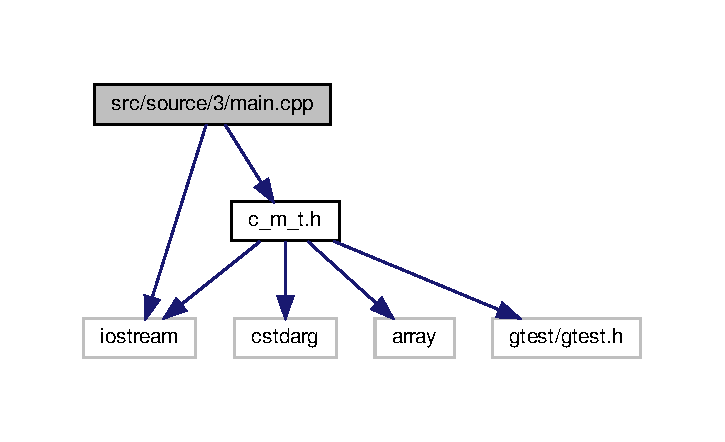
\includegraphics[width=348pt]{main_8cpp__incl}
\end{center}
\end{figure}
\subsection*{Functions}
\begin{DoxyCompactItemize}
\item 
int \hyperlink{main_8cpp_ae66f6b31b5ad750f1fe042a706a4e3d4}{main} ()
\end{DoxyCompactItemize}


\subsection{Function Documentation}
\mbox{\Hypertarget{main_8cpp_ae66f6b31b5ad750f1fe042a706a4e3d4}\label{main_8cpp_ae66f6b31b5ad750f1fe042a706a4e3d4}} 
\index{main.\+cpp@{main.\+cpp}!main@{main}}
\index{main@{main}!main.\+cpp@{main.\+cpp}}
\subsubsection{\texorpdfstring{main()}{main()}}
{\footnotesize\ttfamily int main (\begin{DoxyParamCaption}{ }\end{DoxyParamCaption})}


%--- End generated contents ---

% Index
\backmatter
\newpage
\phantomsection
\clearemptydoublepage
\addcontentsline{toc}{chapter}{Index}
\printindex

\end{document}
